\section{Tema 2}
\subsection{Teoría de colas}
\begin{figure}[H]
\centering
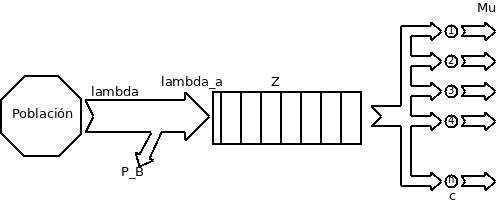
\includegraphics[width=0.9\textwidth]{Imagen/diateocolas.jpg}
\caption{Diagrama teoría de colas}
\label{dia:teocolas}
\end{figure}

\begin{itemize}
	\item $\mu$: Tasa de servicio, velocidad del sistema. Se mide en usuarios por unidad de tiempo.\\
	\item $\lambda$: Tasa de llegadas. Se mide en usuarios por unidad de tiempo.\\
	\item $\lambda_a$:Tasa de llegadas efectiva, la anterior menos los usarios expulsados del sistema. Se mide en usuarios por unidad de tiempo.\\
	\item c: Número de servidores del sistema.\\
	\item Z: Sistema de cola, lo más común FIFO.\\
\end{itemize}
Para analizar el sistema siempre hay que asumir dos cosas: que el sistema no está colapsado y que se está produciendo un reparto uniforme entre todos los servidores.\\
\begin{equation}%[Tráfico ofrecido]
A_o=\frac{E(s)}{E(r)}=\frac{\lambda}{\mu}\text{ E=Tiempo/Tiempo}
\end{equation}
\begin{equation}%[Tráfico cursado]
A_c=A_0(1-P_B)=\frac{\lambda_a}{\mu}\text{ E=Tiempo/Tiempo}
\end{equation}
\begin{equation}%[factor de utilización]
\rho=\frac{A_c}{c}=\frac{\lambda_a}{\mu C}\text{ adimensional}
\end{equation}
\begin{example}
1 petición/hora se resuelve a 1 minuto/petición con una probabilidad de bloqueo 0. Calcula el factor de utilización para 1, 2 y 3 servidores:\\
\[A_o=A_c\]
\[A_o=\frac{\lambda}{\mu}=1\sfrac{pet}{h}1\sfrac{min}{pet}\sfrac{1h}{60min}=\sfrac{1}{60}E=16.7mE\]\\
\[\rho=\frac{A_c}{c}=
\begin{cases}
\sfrac{16.7}{1}=1.67\% & \text{para } c=1\\
\sfrac{16.7}{2}=0.83\% & \text{para } c=2\\
\sfrac{16.7}{3}=0.56\% & \text{para } c=3
\end{cases}\]
\end{example}

\subsubsection{Fórmulas de Little}
Las fórmulas de little son el resultado del análisis de las colas en régimen permanente.
\begin{itemize}
	\item $N(t)$: Número de usuarios en el sistema en un tiempo t.
	\item $N_s(t)$: Número de usuarios en los servidores en un tiempo t.
	\item $N_q(t)$: Número de usuarios en la cola en un tiempo t.
\end{itemize}
\begin{align}%[Fórmulas de little]
N=N_s+N_q\to L &=L_s+L_q\to W=W_s+W_q\\
L_x &=\gamma W_x\\
W_s=E(s)=\sfrac{1}{\mu} & \Leftrightarrow L_s=A_c\\
\gamma &=\lambda_a
\end{align}
\subsubsection{Distribución exponencial}
\begin{figure}[H]
\centering
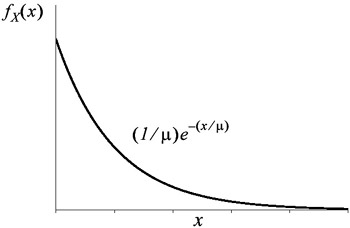
\includegraphics[width=0.9\textwidth]{Imagen/distribucionexponencial.jpg}
\caption{Distribución Exponencial}
\end{figure}
\begin{align}
P(t)=\mu e^{-\mu t} \leftarrow t\geq 0\\
Media=E(s)=\sfrac{1}{\mu}\\
P(t\leq T)=1-e^{-\mu T}
\end{align}
\subsubsection{Distribución de Poisson}
%%Insertar foto de la distribución de Poisson
\begin{figure}[H]
\centering
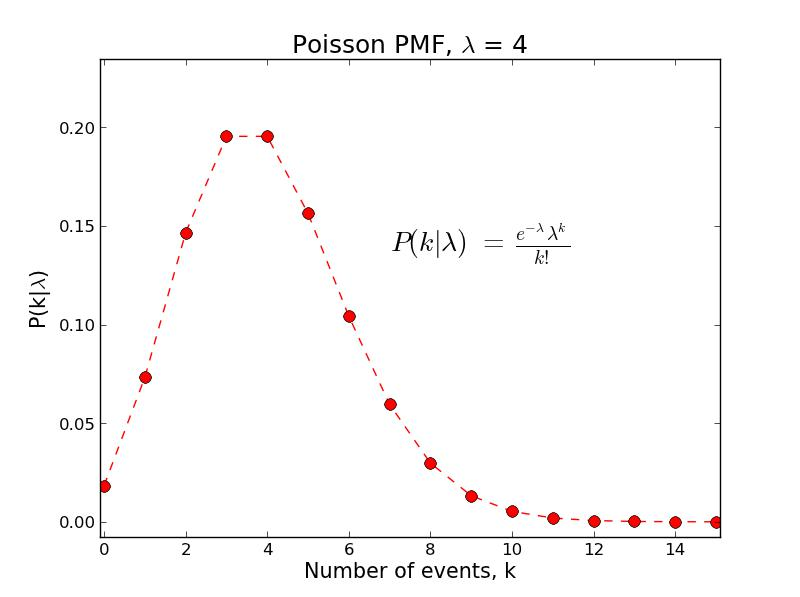
\includegraphics[width=0.9\textwidth]{Imagen/distribucionpoisson.jpg}
\caption{Distribución de Poisson}
\label{}
\end{figure}
\begin{equation}
P(k)=\frac{Ke^{-k}}{K!}
\end{equation}
\subsubsection{Nomenclatura teoría de colas}
\begin{center}
\framebox[1.1\width]{\huge{A/B/c/k/m/Z}} \par
\end{center}
\begin{itemize}
\item {A:} tiempo entre llegadas. m es la distribución normal(Poissoniana), i un modelo determinista y gi es el modelo general.
\item {B:} tasa de servicio. m es la distribución normal(Exponencial), i un modelo determinista y gi es el modelo general.
\item {c:} número de servidores.
\item {k:} capacidad del sistema. En caso de no venir especificado se asume capacidad "infinita".
\item {m:} tamaño de la población. En caso de no venir especificado se asume población "infinita".
\item {Z:} disciplina de la cola. En caso de no venir especificado se asume una cola FIFO.
\end{itemize}
Cuando se habla de poblaciones o capacidades infinitas en realidad significa que el número es mucho mayor que el número de servidores. Población/Capacidad>>c.
\subsubsection{Modelo M/M/1}
Un modelo con llegadas poissonianas, tasa de servicio exponencial, 1 único servidor, una cola infinita, población infinita y una cola con disciplina FIFO. Este modelo tiene una probabilidad de bloqueo nula $P_B=0$ con lo cual se cumple lo siguiente: $A_c=A_o=\sfrac{\lambda}{\mu}$. Al tener un solo servidor además se ve que $\rho=A_o$.
\begin{example}[M/M/1]
Tasa de llegadas 30$\sfrac{\text{clientes}}{\text{hora}}$ con una tasa de servicio de 115$\sfrac{\text{segundos}}{\text{cliente}}$ en un único servidor.
\[A_c=A_o=\frac{\lambda}{\mu}=30*115\sfrac{1}{3600}=0.9583E\] \\
\[\rho=A_c=A_0=0.9583=95.83\%\] Como se puede ver el servidor está a punto de saturarse.\\
\[L=\frac{\rho}{1-\rho}=23\text{ usuarios en el sistema de media}\]
\[L=\frac{\rho^2}{1-\rho}=22\text{ usuarios en la cola de media}\]
\[W=\frac{E(s)}{1-\rho}=45.96\text{ minutos en el sistema de media}\]
\[W=\frac{\rho E(s)}{1-\rho}=44.06\text{ minutos en la cola de media}\]
Los usuarios se quejarán. Hay que esperar 44 minutos en la cola para un servicio que tarda 2 en ser servido.
\end{example}
\subsubsection{Modelo M/M/c}
Un modelo con llegadas poissonianas, tasa de servicio exponencial, c servidores idénticos, una cola infinita, población infinita y una cola con disciplina FIFO. Este modelo tiene una probabilidad de bloqueo nula $P_B=0$ con lo cual se cumple lo siguiente: $A_c=A_o=\sfrac{\lambda}{\mu}$.\\
\begin{example}[M/M/c]
Continuando el ejemplo anterior. $\lambda=\sfrac{\text{clientes}}{\text{hora}}$ con una media de tiempo de servicio $\text{E(s)}=\sfrac{1}{\mu}=115\sfrac{\text{segundos}}{\text{cliente}}$. Contamos con 2 sevidores en lugar de uno. Compararlo con el anterior: W=46min $\text{W}_{\text{q}}$=44min\\
\begin{gather*}
A_o=\frac{\lambda}{\mu}=0.9583E=A_c\\
\rho=\frac{A_c}{c}=0.47915\simeq 48\% \\
L_q=\frac{\rho C(A_o,c)}{(1-\rho)}=0.28\text{ clientes en la cola de media}\\
W_q=\frac{E(s)C(A_o,c)}{c(1-\rho)}=34.2\text{ segundos en la cola de media}
\end{gather*}
Se puede ver una gran mejoría entre los 44 minutos con un único servidor y los 34 segundos en el caso de dos servidores.
\end{example}
\subsubsection{Modelo M/M/c/c}
Un modelo con llegadas poissonianas, tasa de servicio exponencial, c servidores idénticos, sin colas, población infinita y una cola con disciplina FIFO. En este modelo es en el primero que vemos una probabilidad de bloqueo distinta de cero, $P_B=B(A_o,c)$ esta probabilidad se puede calcular gráficamente con las gráficas del Erlang B. En cambio aplicando esto a las fórmulas de little podemos ver lo siguiente: $L_q=0\to L=L_s=A_c=A_o(1-P_B)$\\
\begin{example}[M/M/c/c]
8 servidores con $E(s)=\sfrac{1}{\mu}=4\sfrac{\text{h}}{\text{usuario}}$ y una tasa de llegadas $\lambda=3\sfrac{\text{usuarios}}{\text{h}}$\\
\begin{gather*}
A_o=\frac{\lambda}{\mu}=12E\\
P_B=B(12,8)=42\%
\end{gather*}
\end{example}
\subsubsection{Ejercicios}
\begin{exercise}[1]
Se desea estudiar el envío de paquetes de 128 bytes en una red de conmutación de paquetes con encaminamiento fijo. El enlace entre nodos tiene una capacidad de 64kbps.\\
\textbf{1.} ¿Qué modelo de sistema de colas se puede aplicar?.\\
Se trata de un sistema M/M/1\\
\textbf{2.} ¿Cuál es el número medio de paquetes servidos por segundo?\\
\[\mu=8\sfrac{KB}{s}\frac{1Paquete}{128Bytes}=62.5\sfrac{Paquetes}{s}\]
\textbf{3.} ¿Cuál es el número medio de paquetes por segundo que un nodo puede aceptar para que el tiempo medio de espera en el buffer sea igual a 10 segundos?\\
\begin{gather*}
W_q=\frac{\rho}{\mu(1-\rho)}=10s\\
\rho=\frac{A_c}{c}=A_o=\frac{\lambda}{\mu}\to \lambda=\rho \mu\\
W_q=\frac{\rho}{\mu(1-\rho)}\to\rho=\frac{W_q \mu}{1+W_q\mu}=0.9984\\
\lambda=62.4\sfrac{Paquetes}{s}
\end{gather*}
\textbf{4.} ¿Cuánta memoria en media se estará ocupando en el nodo?\\
\[\text{Memoria}=L_q128=128\frac{\rho^2}{1-\rho}=79.744kB=637.9kb\]
\[L_q=623 \text{ Paquetes en cola de media}\]
\end{exercise}
\begin{exercise}[2]
Un conmutador monoproceso de servicio 16 horas al día FCFS(First Come First Serve) a un conjunto de usuarios. El patrón de llegadas programadas es poissonianode media 20 programas/día y la distribución de tiempo de CPU  de cada programa es exponendial de media 30 minutos.\\
\textbf{1.} ¿Cuál será el factor de utilización de la CPU?\\
Se trata de un M/M/1 con lo cual $\rho=A_o$.\\
\[\rho=\frac{\lambda}{\mu}=\frac{20*30}{60*16}=0.625=62.5\%\]
\textbf{2.} Se reciben quejas de los usuarios, ¿a qué puede ser debido?\\
\[W_q=\frac{\rho}{\mu(1-\rho)}=50\text{ minutos}\]
Se está casi el doble de tiempo en cola que dentro del servidor. Este será el motivo de queja mayoritario.\\
\textbf{3.} Se decide colocar en paralelo tantas CPUs como sean necesarias para garantizar que el tiempo medio de espera en cola sea inferior o como máximo de 10 minutos. ¿Cuántos deben colocarse?\\
\begin{gather*}
A_c=A_o=0.625\\
\rho=\frac{A_c}{c}=\frac{A_o}{c}\\
W_q=E(s)\frac{C(A_o,c)}{c(1-\rho)}
\end{gather*}
Hallaremos la respuesta por prueba y error:
\begin{center}
\begin{tabular}{c|c|c|c}
CPU & $\rho$ & $C(A_o,c)$ & $W_q$ \\\hline
2 & 0.3125 & 0.15 & 3.27 min\\
3 & 0.208 & 0.03 & 0.38 min
\end{tabular}
\end{center}
Como se puede ver en la tabla con solamente añadir un segundo servidor se puede conseguir el objetivo de estar menos de 10 minutos en la cola.\\
\textbf{4.} ¿Es conveniente instalar 2 CPUs que se repartan los usuarios de forma que cada una atienda por separado a la mitad de las peticiones recibidas?\\
Aquí se puede ver que vuelve a ser un sistema M/M/1 con $\lambda=10\sfrac{programas}{dia}$.
\begin{gather*}
\rho=A_o=\frac{\lambda}{\mu}=\frac{30*10}{60*16}=0.3125\\
W_q=E(s)\frac{\rho}{1-\rho}=13.63 \text{ minutos de espera de media}
\end{gather*}
Como se puede ver 13.63\textgreater \textgreater 3.27. Con esto se demuestra que los sistemas de cola única son mucho más eficientes.
\end{exercise}
\begin{exercise}[3]
Los usuarios de una población infinita demandan poisonianamente con tasa 0.1 demandas/segundo un recurso sin cola de espera, con c servidores idénticos. El servicio demandado es exponencial de media E(s). Se desea garantizar que el tiempo de respuesta no sea superior a 10 segundos para al menos el 80\% de los usuarios, y se quiere perder menos del 15\% de los usuarios.\\
\textbf{1.} Calcular E(s) para cumplir con los valores requeridos.\\
\begin{gather*}
p(t<10s)=1-e^{-10\mu}=0.8 \to \mu=0.16\sfrac{\text{demandas}}{\text{segundo}}\\
E(s)=\frac{1}{\mu}=6.25\sfrac{\text{s}}{\text{demanda}}
\end{gather*}
\textbf{2.} ¿Cuántos servidores es necesario colocar?\\
Con $A_o=\sfrac{\lambda}{\mu}=0.625E$ y $P_B<15\%$ miramos en la gráfica de Erlang B y obtenemos que el número de servidores c ha de ser mayor o igual a 2.\\
\textbf{3.} ¿Cuántos servidores están desocupados en media?\\
$L=L_s=A_c=A_o(1-P_B)=0.53125$ usuarios de media en el sistema con lo cual hay 1.46875 servidores libres de media en el sistema.
\end{exercise}